\chapter{Results and Evaluation}
\label{chap:eval}

This chapter presents the results of the experiments conducted using diverse datasets and visualization techniques. The primary focus was to evaluate the effectiveness of the modified t-SimCNE, the hybrid t-SNE with SimCLR, and the standalone t-SNE. The chapter also examines the impact of different loss functions on the quality of data visualization and the ability to discern class separations.

\section{Visualization Outcomes}

Each visualization method was applied to CIFAR-10, Leukemia, Bloodmnist, and Dermamnist datasets:

\begin{figure}[hbt]
\centering
\includegraphics[width=\textwidth]{figs/toy_datasets_tsimcne.png}
\caption{2D embeddings of the datasets using standard t-SimCNE with 150 epochs (which is considered small)
}
\label{fig:med_tsimcne}
\end{figure}

\begin{figure}[hbt]
\centering
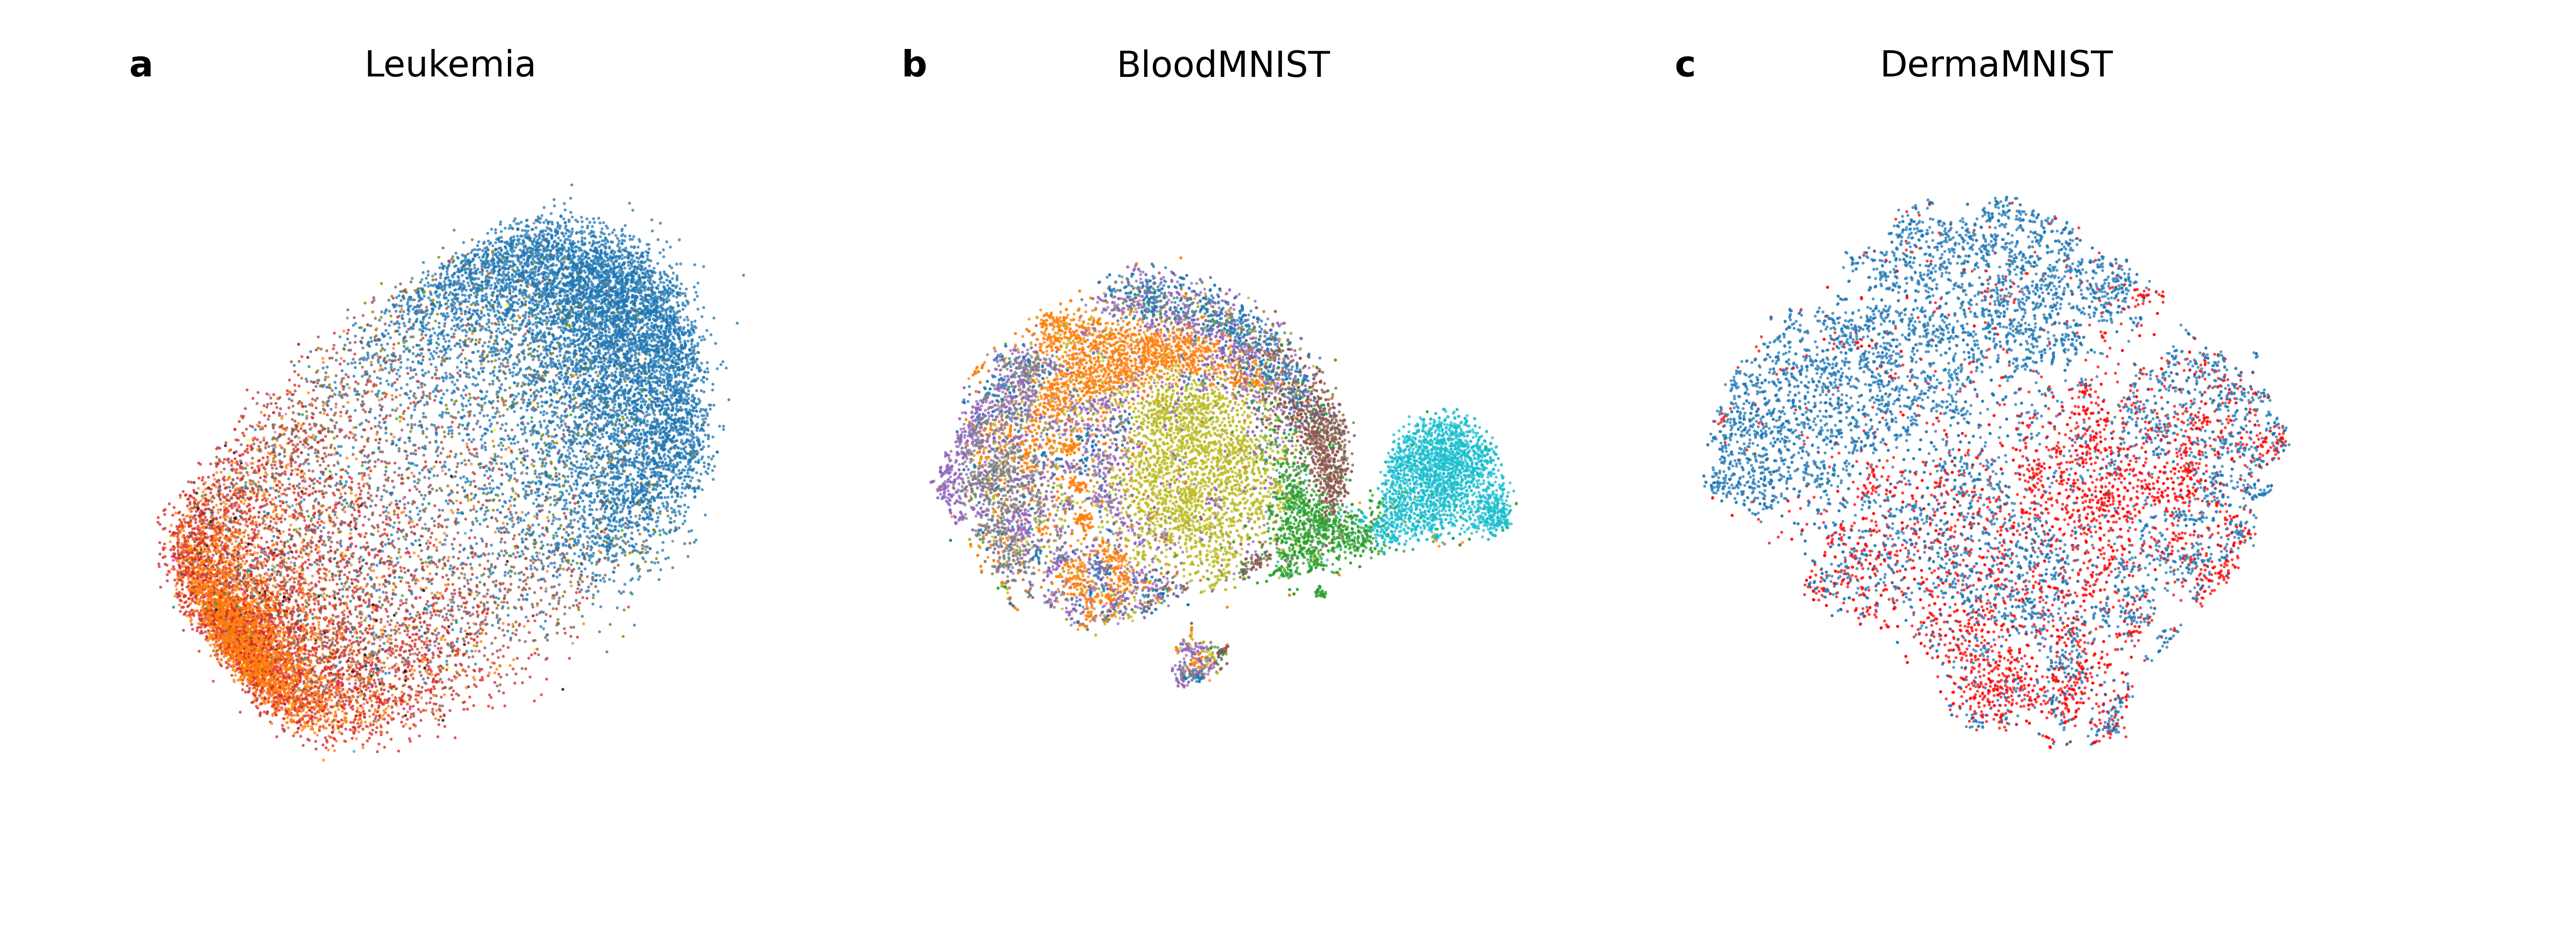
\includegraphics[width=\textwidth]{figs/toy_datasets_tsne.png}
\caption{
2D embeddings of the datasets using t-SNE
}

\label{fig:med_tsne}
\end{figure}

Figure~\ref{fig:med_tsimcne} illustrates the 2D visualizations of learned representations with standard t-SimCNE. It is worth noting that KNN accuracy and overall feature representation quality increases with training, but it requires more computational time and a large number of epochs.

Figure~\ref{fig:med_tsne} illustrates the 2D visualizations with the use of standalone t-SNE without any learning. They may seem to be more accurate visually, discerning the data better, but as Böhm et al. \cite{tsimcne} noted, there are two main problems: 

\begin{itemize}
    \item They don't clearly show details like outliers or different subgroups, making them harder to understand compared to t-SimCNE visualizations
    \item They can't be used to add new images into an already existing visualization, which is something that can be very useful in real-world uses.
\end{itemize}

\begin{figure}[hbt]
\centering
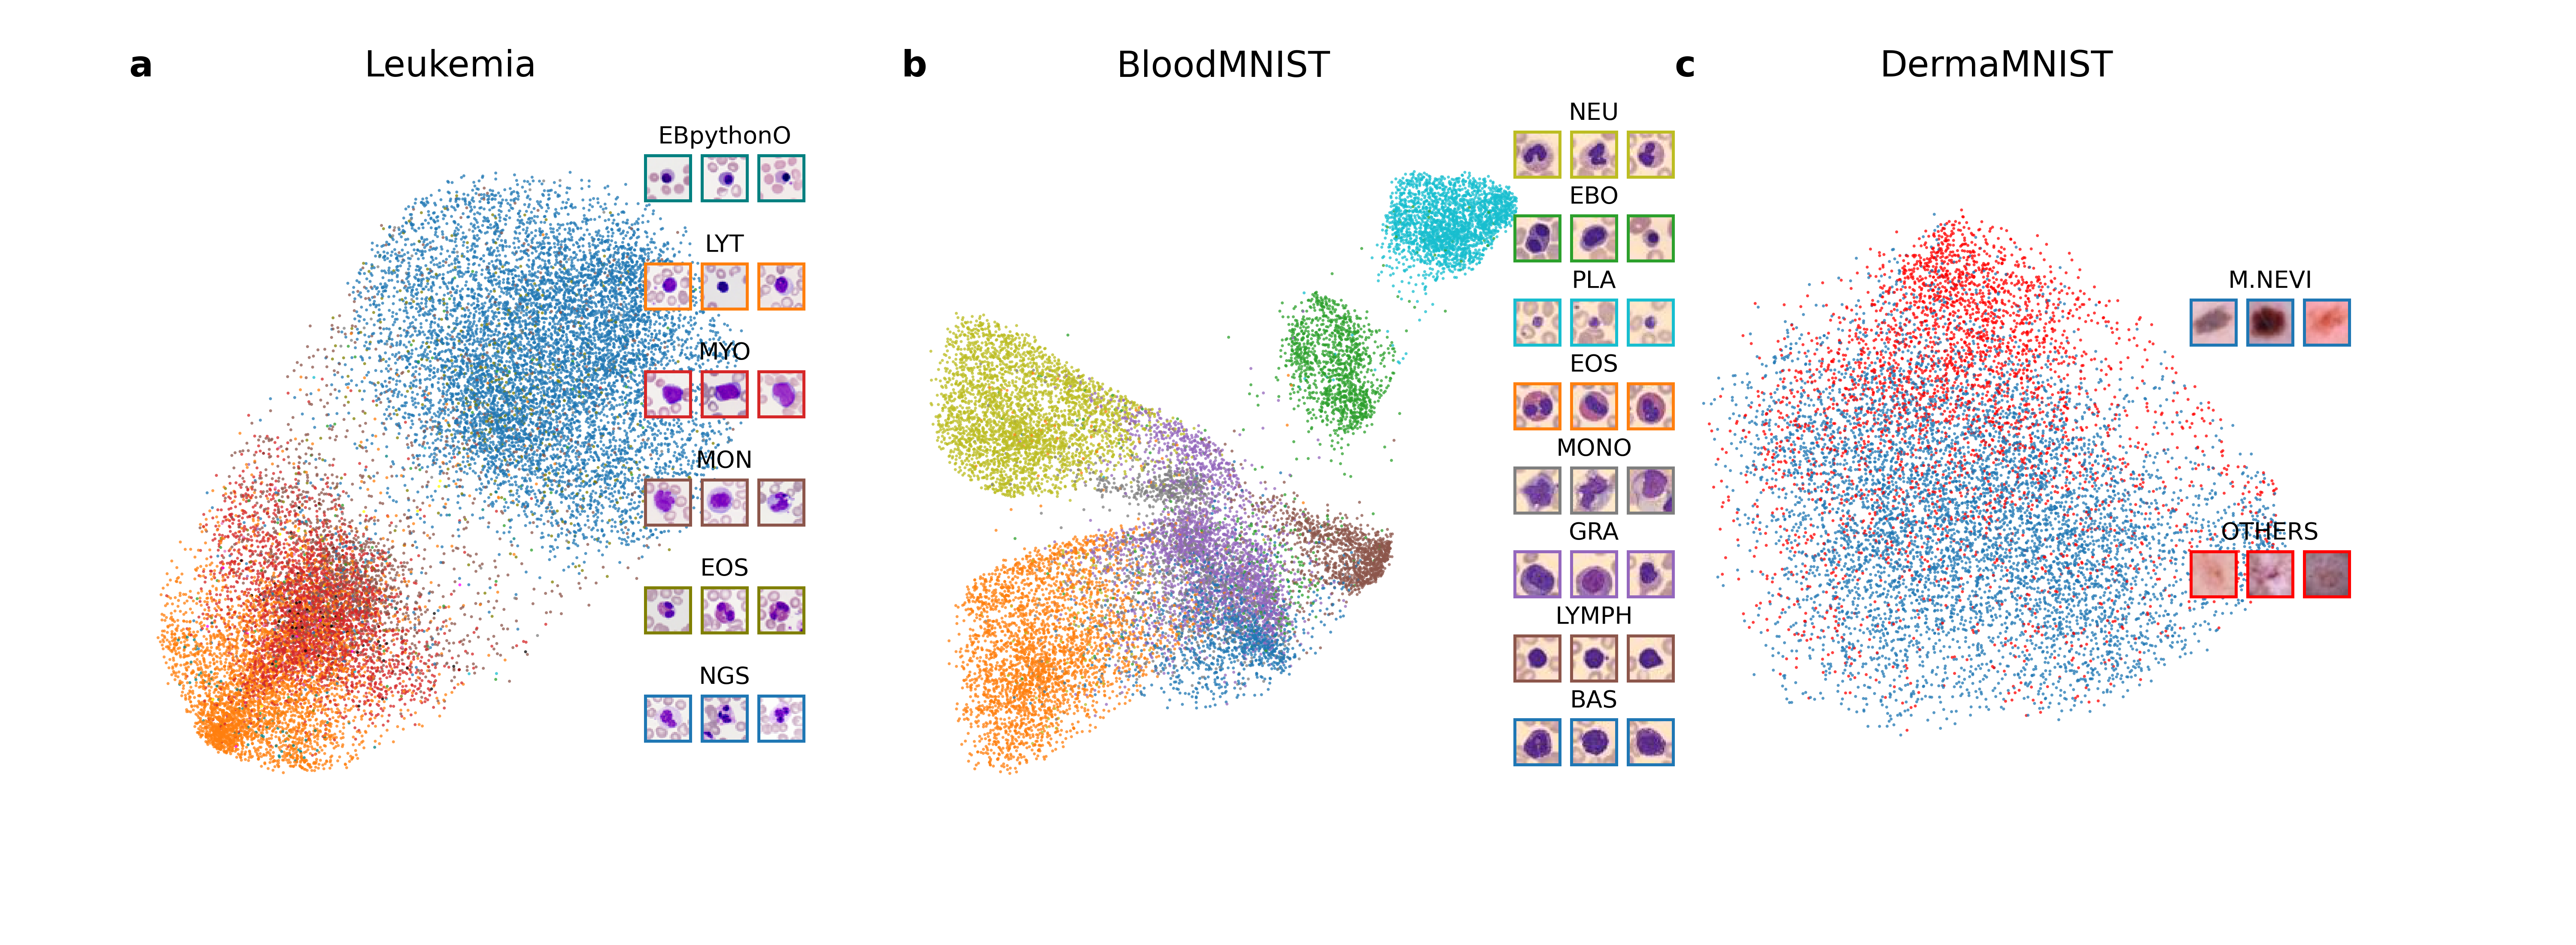
\includegraphics[width=\textwidth]{figs/toy_datasets_long_2.png}
\caption{
2D embeddings of the datasets using our approach with t-SimCNE and AUC-CL
}
\label{fig:tsimcne_auc_cl}
\end{figure}


Unfortunately, our hard negative sampling approach had neither visual nor metrical improvements (Figure~\ref{fig:hardneg}). However, the AUC-CL approach has shown a small rise in performance. Figure~\ref{fig:tsimcne_auc_cl} shows that our implementation of the t-SimCNE algorithm with integration of the AUC-CL approach resulted in a better visual results than both of the previous methods and enhanced ability to discern distinct data clusters more clearly, while using a smaller batch size (256), which requires much less computing power.

\begin{figure}[hbt]
\centering
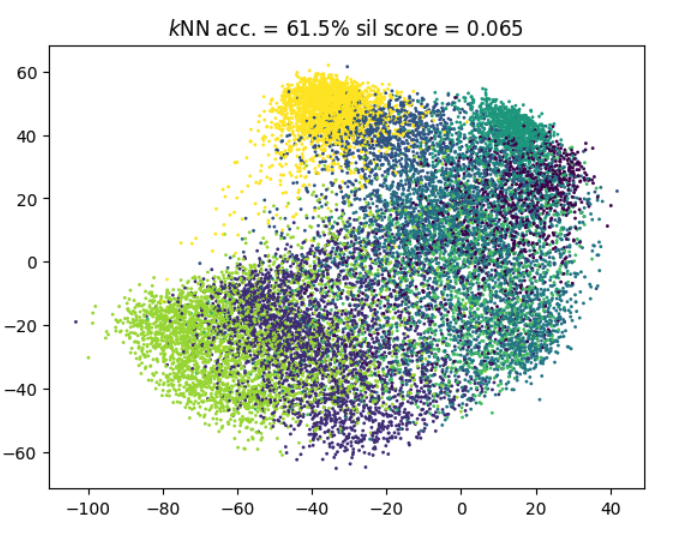
\includegraphics[width=\textwidth]{figs/hardneg.png}
\caption{
Our Hard Negative Sampling approach for CIFAR-10 dataset with 150 epochs.
}
\label{fig:hardneg}
\end{figure}

\subsection{Quantitative Evaluation}

Quantitative metrics were employed to further evaluate the performance of each visualization technique:

\begin{itemize}
    \item {k-NN Classifier}: Used to assess the quality of embeddings by measuring classification accuracy on the low-dimensional data produced by each visualization technique. Results indicate that embeddings from t-SimCNE and t-SNE with SimCLR outperform those from standalone t-SNE.
    \item {Robustness to Batch Size Variations}: Particularly for AUC-CL, we observed minimal loss in accuracy with reduced batch sizes, highlighting its robustness compared to traditional contrastive learning approaches.
\end{itemize}

\begin{figure}[hbt]
\centering
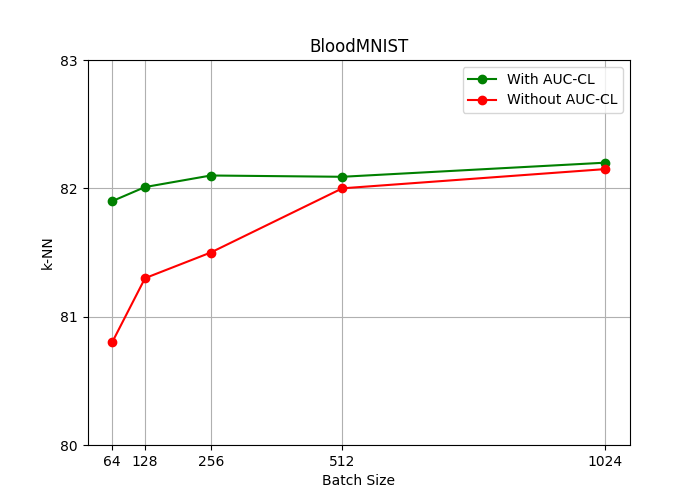
\includegraphics[width=\textwidth]{figs/accuracy_comparison.png}
\caption{
k-NN classifier with different batch sizes using the AUC-CL approach for the BloodMNIST dataset
}
\label{fig:knn_comparison}
\end{figure}


The plot \pic{fig:knn_comparison} shows that the inclusion of AUC-CL in the training process leads to higher k-NN accuracy across all batch sizes. 
Additionally, our method maintains consistent performance across different batch sizes, showing robustness, which can be particularly useful with limited computational resources.



